\section{Padding}
Padding, konvolüsyon sırasında giriş verisinin kenarlarına eklenen ek veri miktarını ifade eder. Bu, çıktı boyutunu kontrol etmek veya giriş verisindeki bilginin kaybolmasını önlemek için kullanılır. İki yaygın tür:

\begin{itemize}
    \item \textbf{Valid Padding:} Kenarlara ek veri eklenmez dolayısıyla çıktı boyutu giriş boyutundan daha küçüktür. Kenar bilgilerinin korunmaya ihtiyaç olmadığı durumlarda ve özellik haritasının boyutunu küçültmek istendiğinde kullanılır.
    \item \textbf{Same Padding:} Giriş verisinin kenarlarına ek veri eklenir böylece çıktı ile giriş aynı boyutta olur. Kenar bilgilerinin korunmaya ihtiyaç olmadığı durumlarda kullanılır.
\end{itemize}

\begin{figure}[h]
    \centering
    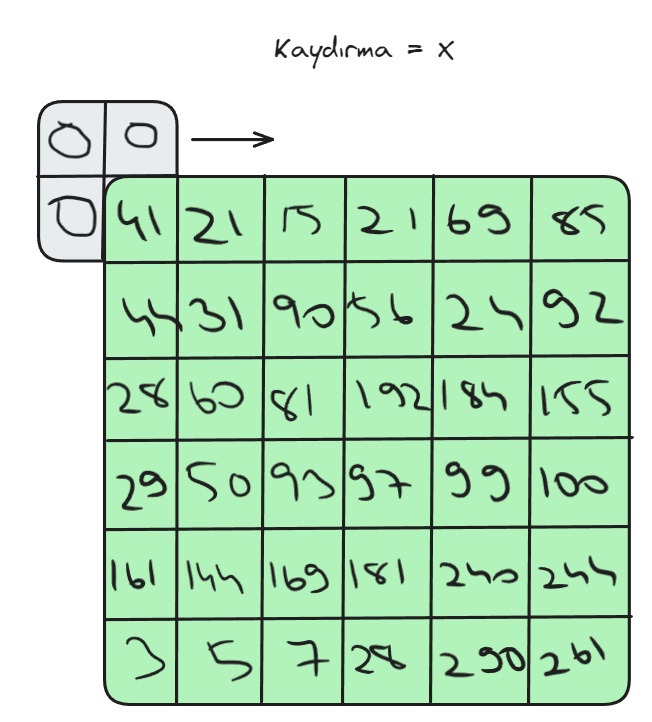
\includegraphics[width=0.7\textwidth]{images/padding_layer.png}
    \caption{Padding katmanı.}
    \label{fig:enter-label}
\end{figure}

\newpage